% Options for packages loaded elsewhere
\PassOptionsToPackage{unicode}{hyperref}
\PassOptionsToPackage{hyphens}{url}
%
\documentclass[
]{article}
\usepackage[dvipsnames]{xcolor}
\usepackage{background}
\usepackage{tikz}
\usepackage[french]{babel}
\usepackage{titletoc}
\usepackage{titlesec}
\usepackage{lipsum}
\usepackage{tocloft}
\usepackage{cancel}
\usepackage{bbold}
\usepackage{algorithm}
\usepackage{algpseudocode}
\usepackage{float}
\usepackage{multirow}
\usepackage{tabularx}
\usepackage{hyperref}
\usepackage{amsmath,amsfonts,amssymb}
\usepackage{color}
\usepackage{xcolor}
\usepackage{enumitem}
\usepackage{mdframed} % Chargement du package mdframed
\usepackage{graphicx}

\renewcommand{\cfttoctitlefont}{\hfill\large\bfseries\fontsize{20}{24}\selectfont}
\renewcommand{\cftaftertoctitle}{\hfill\mbox{}}

\definecolor{mydarkyellow}{HTML}{8B0000}

\backgroundsetup{
	scale=1,
	color=black,
	opacity=0.5,
	angle=0,
	contents={
		\ifnum\value{page}=1
		\begin{tikzpicture}[remember picture,overlay]
			\path [fill=mydarkyellow] (current page.south west) rectangle (current page.north east);
		\end{tikzpicture}
		\fi
	}
}

\title{\textbf{\Huge Polytech Nice}\\[1cm]
	\textbf{\LARGE Création d'un modèle mathématique dans le domaine du sport}\\[2cm]
	\hrule height 1pt
	\vspace{0.5cm}
	\textbf{\Large Étude sur les paramètres qui créent les pics de forme chez un athlète}\\[0.5cm]
	\hrule height 1pt
	\vspace{3cm}
	\small{\today}}


\author{
	\begin{tabular}{c}
		Gerbaud Florent \\
	\end{tabular}
}

\date{}

\begin{document}
	\maketitle
	\newpage
	
	{
		\setcounter{tocdepth}{3}
		% Table des matières
		\renewcommand{\contentsname}{
			\hfill
			\begin{tikzpicture}
				\node[draw, fill=white, inner sep=20pt,line width=1.5pt] {\fontsize{30}{36}\selectfont\bfseries Table des matières};
			\end{tikzpicture}
			\hfill
		}
		\tableofcontents
		\pagebreak
		
	}
	\hypertarget{s1}{%
	\section{Un premier modèle }\label{s1}}
	\hypertarget{ss1}{%
		\subsection{Le premier modèle mathématique }\label{ss1}}
		Dans un premier temps, je me suis concentré sur un système plutôt simple en prenant un nombre d'entrainement par semaine toujours identique (ce qui est plutôt proche de la réalité), une qualité des entrainement par semaine linéaire (plutôt éloigner de la réalité c'est plutôt cyclique) et avec la confiance qui ne dépend que de la qualité des entrainements.
		La partie sur la forme de l'athlète viendra dans une autre partie. 
		\newline\newline 
		\underline{\textbf{Équations théoriques}}
		\newline
		\begin{align*}
			&\text{N(t):="nombre d'entrainement de l'athlète)"} \\
			&\text{C(t):="Confiance de l'athlète"} \\
			&\text{E(t):="qualité des entrainements de l'athlète"}
		\end{align*}
		
		\underline{\textbf{Modèle mathématique}}
		\newline
		\begin{align}
			&N(t+1)=N(t) \\
			&C(t+1)=C(t)+max\{-C(t),E(t)\} \\
			&E(t+1)=E(t)+N(t)(\alpha-\beta) \\
			&\boxed{\begin{array}{c} N(t) \ge 0 \\ C(t) \ge 0 \\
			-1 \le E(t) \le 1\end{array}}
		\end{align}
	
	\underline{\textbf{Les constantes}}
	\newline
	\begin{align}
		&\text{$\alpha$:="la séance a été plus ou moins bien réussie"} \\
		&\text{$\beta$:="Difficulté à récupérer après les séances"}	\end{align}
	
	\hypertarget{ss2}{%
	\subsection{Les premier graphiques }\label{ss2}}
		
		\begin{figure}[H]
			\centering
			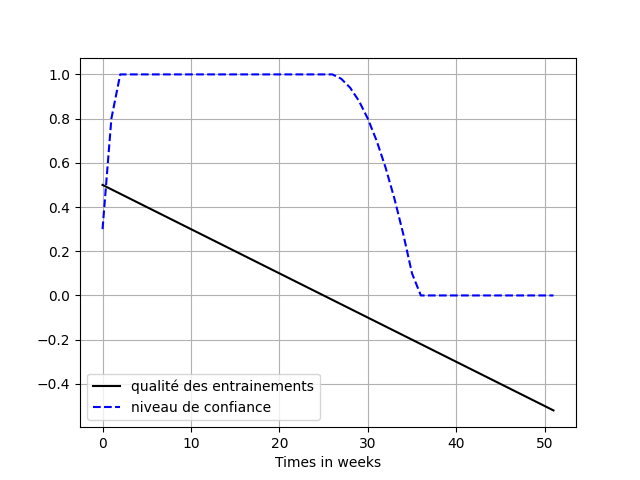
\includegraphics[width=\textwidth]{Graph1SImu1}
			\caption{Un athlète avec peu de confiance et une qualité d'entrainement qui décroit avec le temps}
			\label{fig:fig1_1}
		\end{figure}
		
		\underline{\textbf{Les conditions initiales}}
		\begin{align*}
			\boxed{\begin{array}{c} N_0=\frac{3}{20} \\ E_0=0.5 \\
					C_0=0.3 \\
				\alpha=0.3 \\
				\beta=0.5
				\end{array}}
		\end{align*}
		
		\begin{figure}[H]
			\centering
			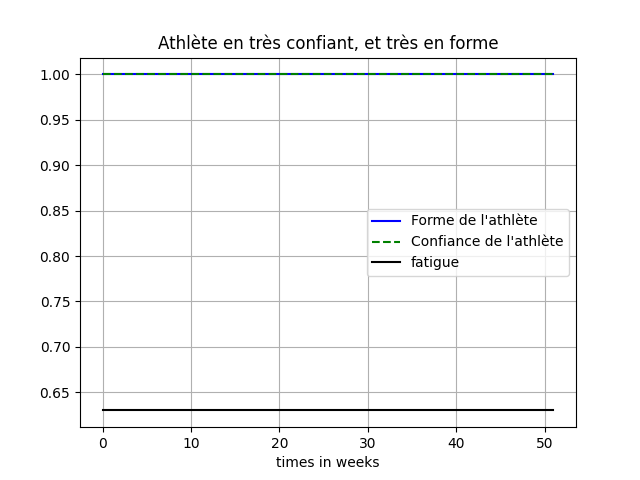
\includegraphics[width=\textwidth]{Graph2SImu1}
			\caption{Un athlète avec peu de confiance et une qualité d'entrainement qui croit avec le temps}
			\label{fig:fig1_3}
		\end{figure}
		
		\underline{\textbf{Les conditions initiales}}
		\begin{align*}
			\boxed{\begin{array}{c} N_0=\frac{3}{20} \\ E_0=0.5 \\
					C_0=0.3 \\
					\alpha=0.7 \\
					\beta=0.5
			\end{array}}
		\end{align*}
		
		\begin{figure}[H]
			\centering
			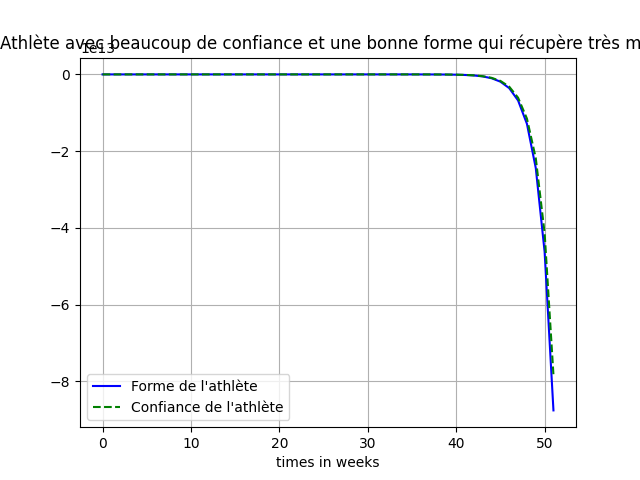
\includegraphics[width=\textwidth]{Graph3SImu1}
			\caption{Un athlète avec beaucoup de confiance et une qualité d'entrainement parfaite}
			\label{fig:1_3}
		\end{figure}
		
		\underline{\textbf{Les conditions initiales}}
		\begin{align*}
			\boxed{\begin{array}{c} N_0=\frac{3}{20} \\ E_0=1 \\
					C_0=1 \\
					\alpha=0.7 \\
					\beta=0.5
			\end{array}}
		\end{align*}
		
		\begin{figure}[H]
			\centering
			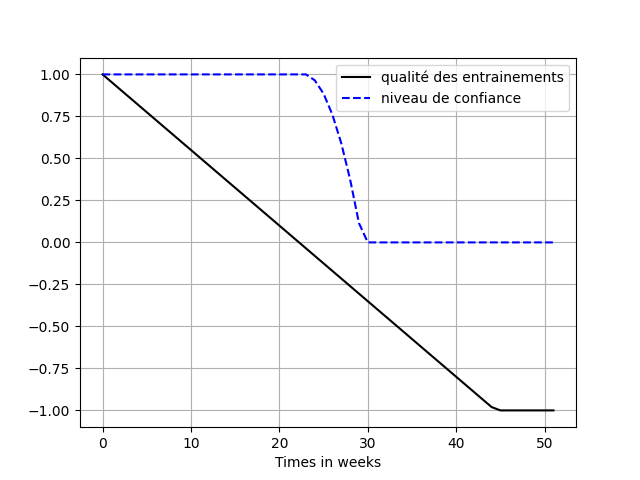
\includegraphics[width=\textwidth]{Graph4SImu1}
			\caption{Un athlète avec beaucoup de confiance et une qualité d'entrainement qui se dégrade}
			\label{fig:1_4}
		\end{figure}
		
		\underline{\textbf{Les conditions initiales}}
		\begin{align*}
			\boxed{\begin{array}{c} N_0=\frac{3}{20} \\ E_0=1 \\
					C_0=1 \\
					\alpha=0.2 \\
					\beta=0.5
			\end{array}}
		\end{align*}
		
		\begin{figure}[H]
			\centering
			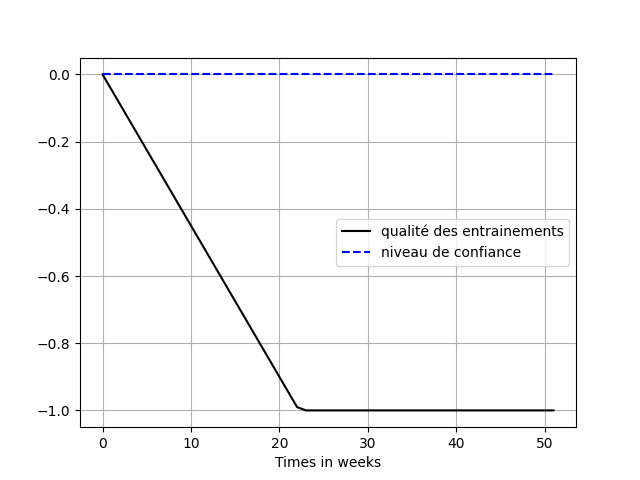
\includegraphics[width=\textwidth]{Graph5SImu1}
			\caption{Un athlète avec aucune confiance et une qualité d'entrainement qui se dégrade}
			\label{fig:1_5}
		\end{figure}
		
		\underline{\textbf{Les conditions initiales}}
		\begin{align*}
			\boxed{\begin{array}{c} N_0=\frac{3}{20} \\ E_0=0 \\
					C_0=0 \\
					\alpha=0.2 \\
					\beta=0.5
			\end{array}}
		\end{align*}
		
		\begin{figure}[H]
			\centering
			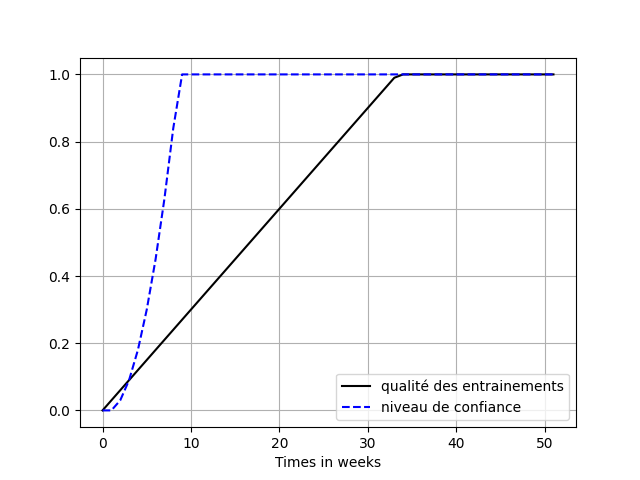
\includegraphics[width=\textwidth]{Graph6SImu1}
			\caption{Un athlète avec aucune confiance et une qualité d'entrainement qui s'améliore}
			\label{fig:1_6}
		\end{figure}
		
		\underline{\textbf{Les conditions initiales}}
		\begin{align*}
			\boxed{\begin{array}{c} N_0=\frac{3}{20} \\ E_0=0 \\
					C_0=0 \\
					\alpha=0.7 \\
					\beta=0.5
			\end{array}}
		\end{align*}
		
		\hypertarget{s2}{%
		\section{Une amélioration du premier modèle }\label{s21}}
		\hypertarget{ss1}{%
		\subsection{Le nouveau modèle mathématique }\label{ss21}}
		\underline{\textbf{Modèle mathématique}}
		\newline
		\begin{align*}
			&N(t+1)=N(t) \\
			&C(t+1)=C(t)+max\{-C(t),E(t)\} \\
			&E(t+1)=E(t)+N(t)(\alpha(t)-\beta(t)) \\
			&\boxed{\begin{array}{c} N(t) \ge 0 \\ C(t) \ge 0 \\
					-1 \le E(t) \le 1\end{array}}
		\end{align*}
		\underline{\textbf{Les constantes}}
		\newline
		\begin{align*}
			&\alpha(t) =\frac{X_t}{N(t)}, \ \text{t=\{1,....,nbSemaine\}}, \ X_t \sim \operatorname{Bin}(N(t),moySeanceValide) \\
			&\beta(t) = \begin{cases}
				\mathcal{U}_t[niveauFatigueMoyen-0.02,niveauFatigueMoyen+0.02] \ si \ X_t=1 \\
				\mathcal{U}_t[0,1] \ sinon
			\end{cases}, \ \ X_t \sim \operatorname{Bin}(1,0.9) \\
			&moySeanceValidee:=\text{"probabilité de réussir en moyenne un certains nombre de séance"} \\
			&niveauFatigueMoyen:=\text{"taux de fatigue moyen généré par une semaine d'entrainement"}
		\end{align*}
		\hypertarget{ss22}{%
		\subsection{Les nouveaux graphiques }\label{ss22}}
		\begin{figure}[H]
			\centering
			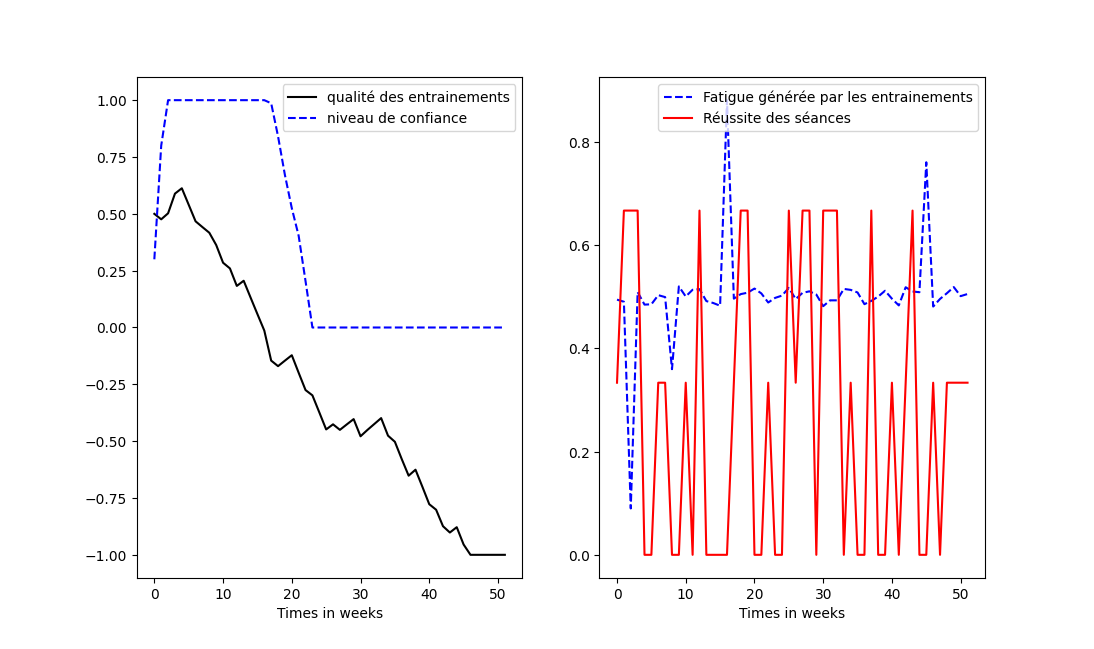
\includegraphics[width=\textwidth]{Graph1SImu2}
			\caption{Un athlète avec peu de confiance et une qualité d'entrainement qui décroit avec le temps}
			\label{fig:2_1}
		\end{figure}
		\underline{\textbf{Les conditions initiales}}
		\begin{align*}
			\boxed{\begin{array}{c} N_0=\frac{3}{20} \\ E_0=0.5 \\
					C_0=0.3 \\
					moySeanceValidee=0.3 \\
					niveauFatigueMoyen=0.5
			\end{array}}
		\end{align*}

		\begin{figure}[H]
			\centering
			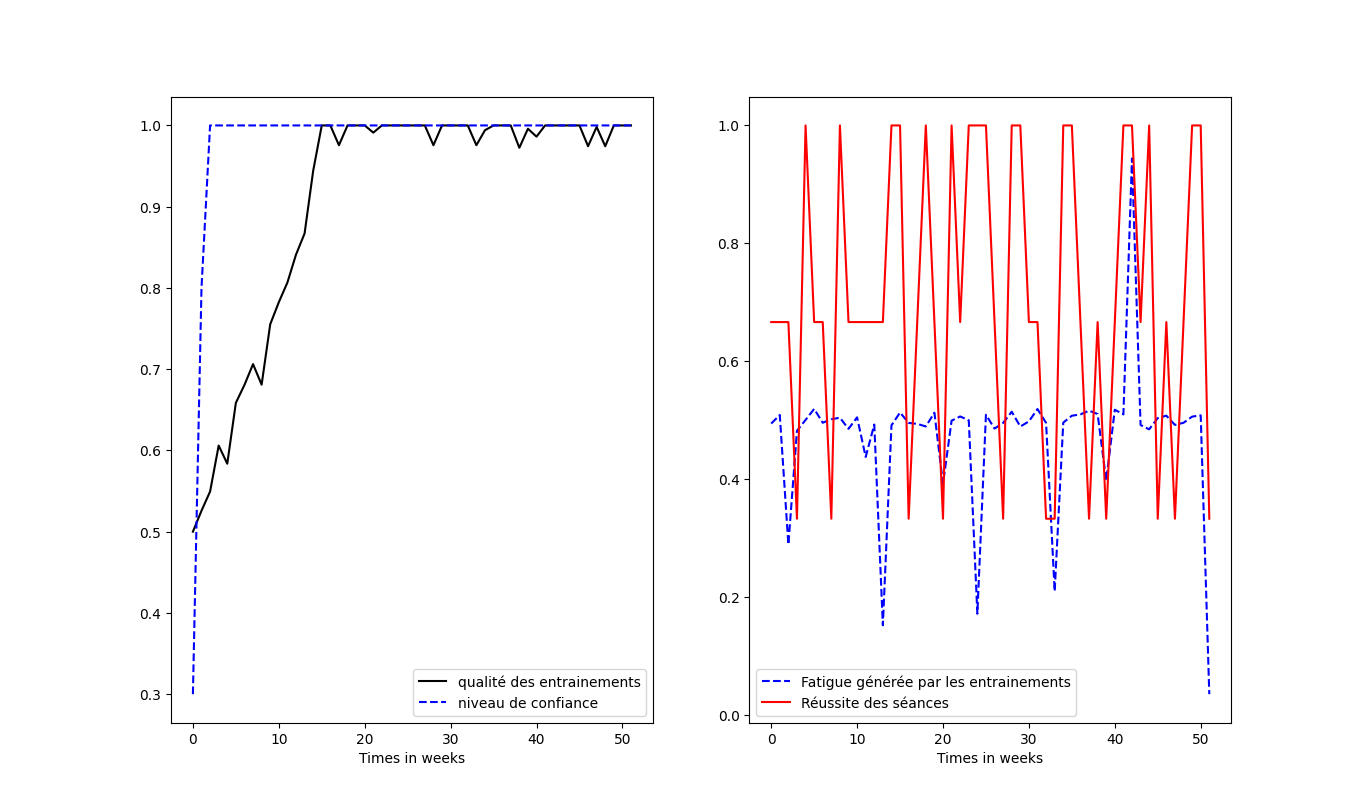
\includegraphics[width=\textwidth]{Graph2SImu2}
			\caption{Un athlète avec peu de confiance et une qualité d'entrainement qui croit avec le temps}
			\label{fig:2_2}
		\end{figure}
		\underline{\textbf{Les conditions initiales}}
		\begin{align*}
			\boxed{\begin{array}{c} N_0=\frac{3}{20} \\ E_0=0.5 \\
					C_0=0.3 \\
					moySeanceValidee=0.7 \\
					niveauFatigueMoyen=0.5
			\end{array}}
		\end{align*}		
\end{document}
